\documentclass[aspectratio=169]{beamer}
\usepackage[utf8]{inputenc}
\usepackage[spanish]{babel}
\usepackage{graphicx}
\usepackage{amsmath}
\usepackage{amsfonts}
\usepackage{tikz}


% --- CONFIGURACIÓN DE COLORES INSTITUCIONALES USS ---
\definecolor{USSBlue}{RGB}{0, 32, 91}    % Azul marino
\definecolor{USSGold}{RGB}{212, 175, 55} % Dorado

\mode<presentation> {
  \usetheme{Madrid}
  \usecolortheme[named=USSBlue]{structure}
  \setbeamercolor{palette primary}{bg=USSBlue,fg=white}
  \setbeamercolor{palette secondary}{bg=USSBlue,fg=white}
  \setbeamercolor{palette tertiary}{bg=USSBlue,fg=white}
  \setbeamercolor{title}{bg=white,fg=USSBlue}
  \setbeamercolor{item}{fg=USSGold}
  \setbeamertemplate{navigation symbols}{} 
}
% --- DATOS DE PORTADA ---
\title[Solemne 2: Cónicas Aplicadas]{Modelamiento Geométrico de Cónicas Aplicado a Navegación Naval y Sistemas Aeroespaciales}
\subtitle{Introducción al Cálculo}
\author[Grupo 3]{Moisés Amundarain, Camila Aravena, Daniela García, Fernando Ramírez, \\ María José Santander, Juan Pablo Vargas}
\institute[USS]{
Ing. Civil Informática e Ing. Civil Industrial \\
  Facultad de Ingeniería \\
  \textbf{Universidad San Sebastián}
}
\date{02 de junio, 2026}

% Logo institucional USS en portada
\titlegraphic{
\includegraphics[width=3cm]{logo_uss.png}}

\begin{document}

% 1. PORTADA PERSONALIZADA CON DISEÑO DE CARD DE TÍTULO SOMBREADA (TIPO BRAZO ROBÓTICO)
\begin{frame}[plain]
  \vspace*{0.3cm}
  \begin{columns}[T]
    \begin{column}{0.48\textwidth}
      
\includegraphics[width=4.6cm]{logo_uss.png}
    \end{column}
    \begin{column}{0.48\textwidth}
      \raggedleft
      \scriptsize \color{black!80}
      Ing. Civil Informática e Ing. Civil Industrial \\
      Facultad de Ingeniería \\
      Universidad San Sebastián \\
      02 de junio, 2026
    \end{column}
  \end{columns}
  
  \vspace{0.4cm}
  \begin{center}
    \begin{beamercolorbox}[sep=10pt, center, rounded=true, shadow=true]{title}
      \centering
      \Large \bfseries \color{USSBlue} Modelamiento Geométrico de Cónicas Aplicado a Navegación Naval y Sistemas Aeroespaciales
      \vspace{0.3cm} \\
      \large \bfseries \color{USSBlue} Introducción al Cálculo
    \end{beamercolorbox}
  \end{center}
  
  \vspace{0.3cm}
  \begin{columns}[T]
    \begin{column}{0.48\textwidth}
      \scriptsize \color{black}
      \textbf{Integrantes (Grupo 3):} \\
      Moisés Amundarain \\
      Camila Aravena \\
      Daniela García
    \end{column}
    \begin{column}{0.48\textwidth}
      \scriptsize \color{black}
      \quad \\
      Fernando Ramírez \\
      María José Santander \\
      Juan Pablo Vargas
    \end{column}
  \end{columns}
\end{frame}

% 2. ORGANIZACIÓN DEL EQUIPO Y DISTRIBUCIÓN DE APORTES
\begin{frame}{Organización del Equipo y Aportes}
  \begin{columns}[T]
    \begin{column}{0.48\textwidth}
      \begin{block}{Problema I: Navegación Naval}
        \scriptsize
        \begin{itemize}
          \item \textbf{Marco Teórico:} Moisés Amundarain
          \item \textbf{Construcción GeoGebra:} Camila Aravena
          \item \textbf{Desarrollo y Preguntas:} Fernando Ramírez y Juan Pablo Vargas
        \end{itemize}
      \end{block}
      \vspace{0.1cm}
      \begin{block}{Problema II: Radioterapia}
        \scriptsize
        \begin{itemize}
          \item \textbf{Marco Teórico:} Moisés Amundarain
          \item \textbf{Construcción GeoGebra:} Camila Aravena
          \item \textbf{Desarrollo y Preguntas:} María José Santander y Daniela García
        \end{itemize}
      \end{block}
    \end{column}
    \begin{column}{0.48\textwidth}
      \begin{block}{Problema III: Órbitas Aeroespaciales}
        \scriptsize
        \begin{itemize}
          \item \textbf{Investigación de Cónicas:} Moisés Amundarain y Camila Aravena
          \item \textbf{Contexto y Desarrollo:} Moisés Amundarain y Camila Aravena
          \item \textbf{Modelamiento (GeoGebra):} Camila Aravena
        \end{itemize}
      \end{block}
      \vspace{0.1cm}
      \begin{block}{Presentación}
        \scriptsize
        \begin{itemize}
          \item \textbf{Diseño y Estructuración Beamer:} Moisés Amundarain
          \item \textbf{Apoyo y Contenido Visual:} Daniela García
        \end{itemize}
      \end{block}
    \end{column}
  \end{columns}
\end{frame}


% 2. ESTRUCTURA Y PUNTOS DE LA EXPOSICIÓN (Sin logo, simple)
\begin{frame}{Estructura y Puntos de la Exposición}
  En esta presentación grupal se abordan el modelamiento geométrico y la resolución analítica de dos problemas reales:
  \vspace{0.4cm}
  \begin{itemize}
    \item \textbf{Problema I: Navegación Táctica de un Submarino}
      \begin{itemize}
        \item Análisis de posición relativa recta-circunferencia.
        \item Determinación de cuerdas de peligro y su significado físico.
        \item Simulación paramétrica en GeoGebra y telemetría de sonar móvil.
      \end{itemize}
    \vspace{0.3cm}
    \item \textbf{Problema III: Sistema de Posicionamiento Aeroespacial y Órbitas}
      \begin{itemize}
        \item Contexto operacional de órbitas cruzadas en el espacio profundo.
        \item Deducción de ecuaciones canónicas para órbitas recíprocas (elipse-hipérbola).
        \item Intersección analítica y cálculo de ventanas de vuelo seguras.
        \item Análisis dinámico de excentricidad orbital y tangencia límite.
      \end{itemize}
  \end{itemize}
\end{frame}

% 3. PROBLEMA I: CONTEXTO Y PLANTEAMIENTO NAVAL
\begin{frame}{Problema I: Contexto y Supuestos Operacionales}
  \begin{columns}[c]
    \begin{column}{0.53\textwidth}
      \textbf{Navegación en Zonas de Peligro:}
      \vspace{0.2cm}
      \scriptsize
      \begin{itemize}
        \item \textbf{Trayectoria del submarino ($\ell$):} Desplazamiento lineal rectilíneo modelado por:
          \[\ell \colon 3x - 4y + 20 = 0\]
        \item \textbf{Campo de minas (Cónica 1):} Obstáculo circular con radio de exclusión $R = 8\text{~km}$, centrado en $M(2, -1)$.
        \item \textbf{Arrecife de coral (Cónica 2):} Obstáculo circular con radio de exclusión $R_A = 5\text{~km}$, centrado en $A(5, 4)$.
      \end{itemize}
    \end{column}
    \begin{column}{0.44\textwidth}
      \centering
      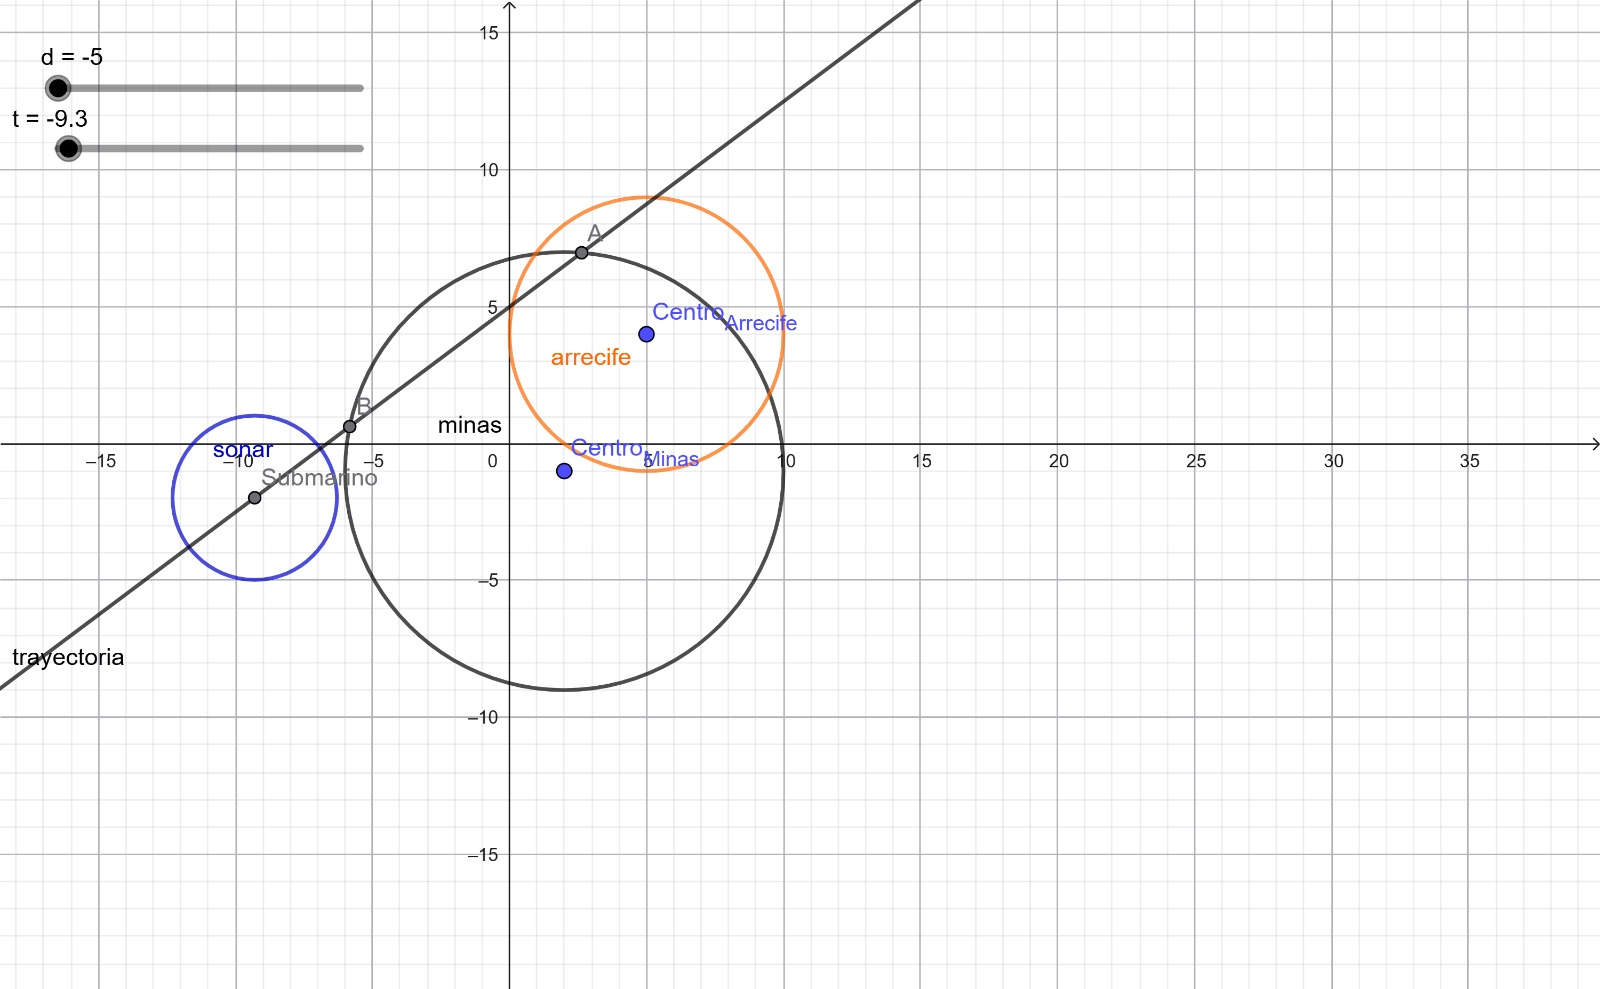
\includegraphics[width=\textwidth,keepaspectratio]{simulacion_naval.jpeg}
      \vspace{0.1cm}
      
      \textit{\scriptsize Simulación del Entorno de Navegación}
    \end{column}
  \end{columns}
\end{frame}

% --- DIAPOSITIVA DE APOYO VISUAL: POSICIONES RELATIVAS ---
\begin{frame}{Problema I: Posiciones Relativas en el Plano}
  \centering
  \small
  El análisis táctico se basa en la clasificación de las posiciones relativas entre la trayectoria $\ell$ y los obstáculos circulares de centro $C$ y radio $R$:
  \vspace{0.3cm}

  \begin{columns}[T]
    \begin{column}{0.31\textwidth}
      \begin{block}{\centering Secante ($d < R$)}
        \centering
        \scriptsize
        La recta corta en dos puntos.\\
        \textbf{Zona de peligro activa.}
        \vspace{0.2cm}
        
        \begin{tikzpicture}[scale=0.9, >=stealth]
          \draw[thick, fill=USSBlue!5] (0,0) circle (1);
          \draw[thick, gray, ->] (0,0) -- (45:1) node[midway, above left] {\tiny $R$};
          \draw[thick, red] (-1.3, 0.5) -- (1.3, 0.5) node[right] {\tiny $\ell$};
          \draw[thick, blue, ->] (0,0) -- (0, 0.5) node[midway, left] {\tiny $d$};
          \fill (0,0) circle (0.04) node[below] {\tiny $C$};
          \fill[red] (-0.866, 0.5) circle (0.04);
          \fill[red] (0.866, 0.5) circle (0.04);
        \end{tikzpicture}
      \end{block}
    \end{column}
    
    \begin{column}{0.31\textwidth}
      \begin{block}{\centering Tangente ($d = R$)}
        \centering
        \scriptsize
        La recta toca en un único punto.\\
        \textbf{Umbral límite / Margen nulo.}
        \vspace{0.2cm}
        
        \begin{tikzpicture}[scale=0.9, >=stealth]
          \draw[thick, fill=USSBlue!5] (0,0) circle (1);
          \draw[thick, gray, ->] (0,0) -- (-45:1) node[midway, below left] {\tiny $R$};
          \draw[thick, red] (-1.3, 1) -- (1.3, 1) node[right] {\tiny $\ell$};
          \draw[thick, blue, ->] (0,0) -- (0, 1) node[midway, left] {\tiny $d$};
          \fill (0,0) circle (0.04) node[below] {\tiny $C$};
          \fill[red] (0, 1) circle (0.04);
        \end{tikzpicture}
      \end{block}
    \end{column}
    
    \begin{column}{0.31\textwidth}
      \begin{block}{\centering Exterior ($d > R$)}
        \centering
        \scriptsize
        La recta no toca la frontera.\\
        \textbf{Ruta segura de navegación.}
        \vspace{0.2cm}
        
        \begin{tikzpicture}[scale=0.9, >=stealth]
          \draw[thick, fill=USSBlue!5] (0,0) circle (1);
          \draw[thick, gray, ->] (0,0) -- (225:1) node[midway, above right] {\tiny $R$};
          \draw[thick, red] (-1.3, 1.4) -- (1.3, 1.4) node[right] {\tiny $\ell$};
          \draw[thick, blue, ->] (0,0) -- (0, 1.4) node[midway, left] {\tiny $d$};
          \fill (0,0) circle (0.04) node[below] {\tiny $C$};
        \end{tikzpicture}
      \end{block}
    \end{column}
  \end{columns}
\end{frame}


% 4. PROBLEMA I: DISTANCIA AL CAMPO DE MINAS
\begin{frame}{Problema I: Aproximación Mínima a las Minas}
  \begin{block}{Fórmula de Distancia de un Punto a una Recta}
    \[d(P_0, \ell) = \frac{|Ax_0 + By_0 + C|}{\sqrt{A^2 + B^2}}\]
  \end{block}
  \vspace{0.3cm}
  \textbf{Cálculo de la Distancia al Centro de las Minas $M(2, -1)$:}
  \[d_1 = \frac{|3(2) - 4(-1) + 20|}{\sqrt{3^2 + (-4)^2}} = \frac{|6 + 4 + 20|}{5} = \frac{30}{5} = 6\text{~km}\]
  \vspace{0.2cm}
  {\centering \textbf{Resultado:} Como $d_1 = 6\text{~km} < R = 8\text{~km}$, la trayectoria es \textbf{secante}. El submarino penetra físicamente en el campo de minas. \par}
\end{frame}


% 5. PROBLEMA I: DISTANCIA AL ARRECIFE DE CORAL
\begin{frame}{Problema I: Aproximación Mínima al Arrecife}
  \begin{block}{Fórmula de Distancia de un Punto a una Recta}
    \[d(P_0, \ell) = \frac{|Ax_0 + By_0 + C|}{\sqrt{A^2 + B^2}}\]
  \end{block}
  \vspace{0.3cm}
  \textbf{Cálculo de la Distancia al Centro del Arrecife $A(5, 4)$:}
  \[d_2 = \frac{|3(5) - 4(4) + 20|}{\sqrt{3^2 + (-4)^2}} = \frac{|15 - 16 + 20|}{5} = \frac{19}{5} = 3.8\text{~km}\]
  \vspace{0.2cm}
  {\centering \textbf{Resultado:} Como $d_2 = 3.8\text{~km} < R_A = 5\text{~km}$, la trayectoria es \textbf{secante}. El submarino ingresa directamente en la zona del arrecife. \par}
\end{frame}

% 7. PROBLEMA I: CUERDA SECANTE EN EL CAMPO DE MINAS
\begin{frame}{Problema I: Cuerda en el Campo de Minas}
  \begin{block}{Fórmula de la Cuerda Secante (Teorema de Pitágoras)}
    \[L = 2\sqrt{R^2 - d^2}\]
  \end{block}
  \vspace{0.3cm}
  \textbf{Cálculo del Tramo Expuesto a las Minas ($R = 8\text{~km}$, $d_1 = 6\text{~km}$):}
  \[L_1 = 2\sqrt{8^2 - 6^2} = 2\sqrt{64 - 36} = 2\sqrt{28} = 4\sqrt{7} \approx 10.58\text{~km}\]
  \vspace{0.3cm}
  \textbf{Significado Físico Naval:}
  Define la distancia lineal exacta ($10.58\text{~km}$) a lo largo de la cual la tripulación se encontrará expuesta de forma directa a la amenaza de las minas submarinas.
\end{frame}

% 8. PROBLEMA I: CUERDA SECANTE EN EL ARRECIFE DE CORAL
\begin{frame}{Problema I: Cuerda en el Arrecife de Coral}
  \begin{block}{Fórmula de la Cuerda Secante (Teorema de Pitágoras)}
    \[L = 2\sqrt{R^2 - d^2}\]
  \end{block}
  \vspace{0.3cm}
  \textbf{Cálculo del Tramo Expuesto al Arrecife ($R_A = 5\text{~km}$, $d_2 = 3.8\text{~km}$):}
  \[L_2 = 2\sqrt{5^2 - 3.8^2} = 2\sqrt{25 - 14.44} = 2\sqrt{10.56} \approx 6.50\text{~km}\]
  \vspace{0.3cm}
  \textbf{Significado Físico Naval:}
  Representa el tramo continuo de $6.50\text{~km}$ de navegación del submarino dentro del arrecife de coral, lo que representa un riesgo crítico de encallamiento por colisión estructural.
\end{frame}

% 6. PROBLEMA I: PLANO DE NAVEGACIÓN (SOPORTE VISUAL)
\begin{frame}{Problema I: Plano de Navegación Táctica}
  \begin{center}
    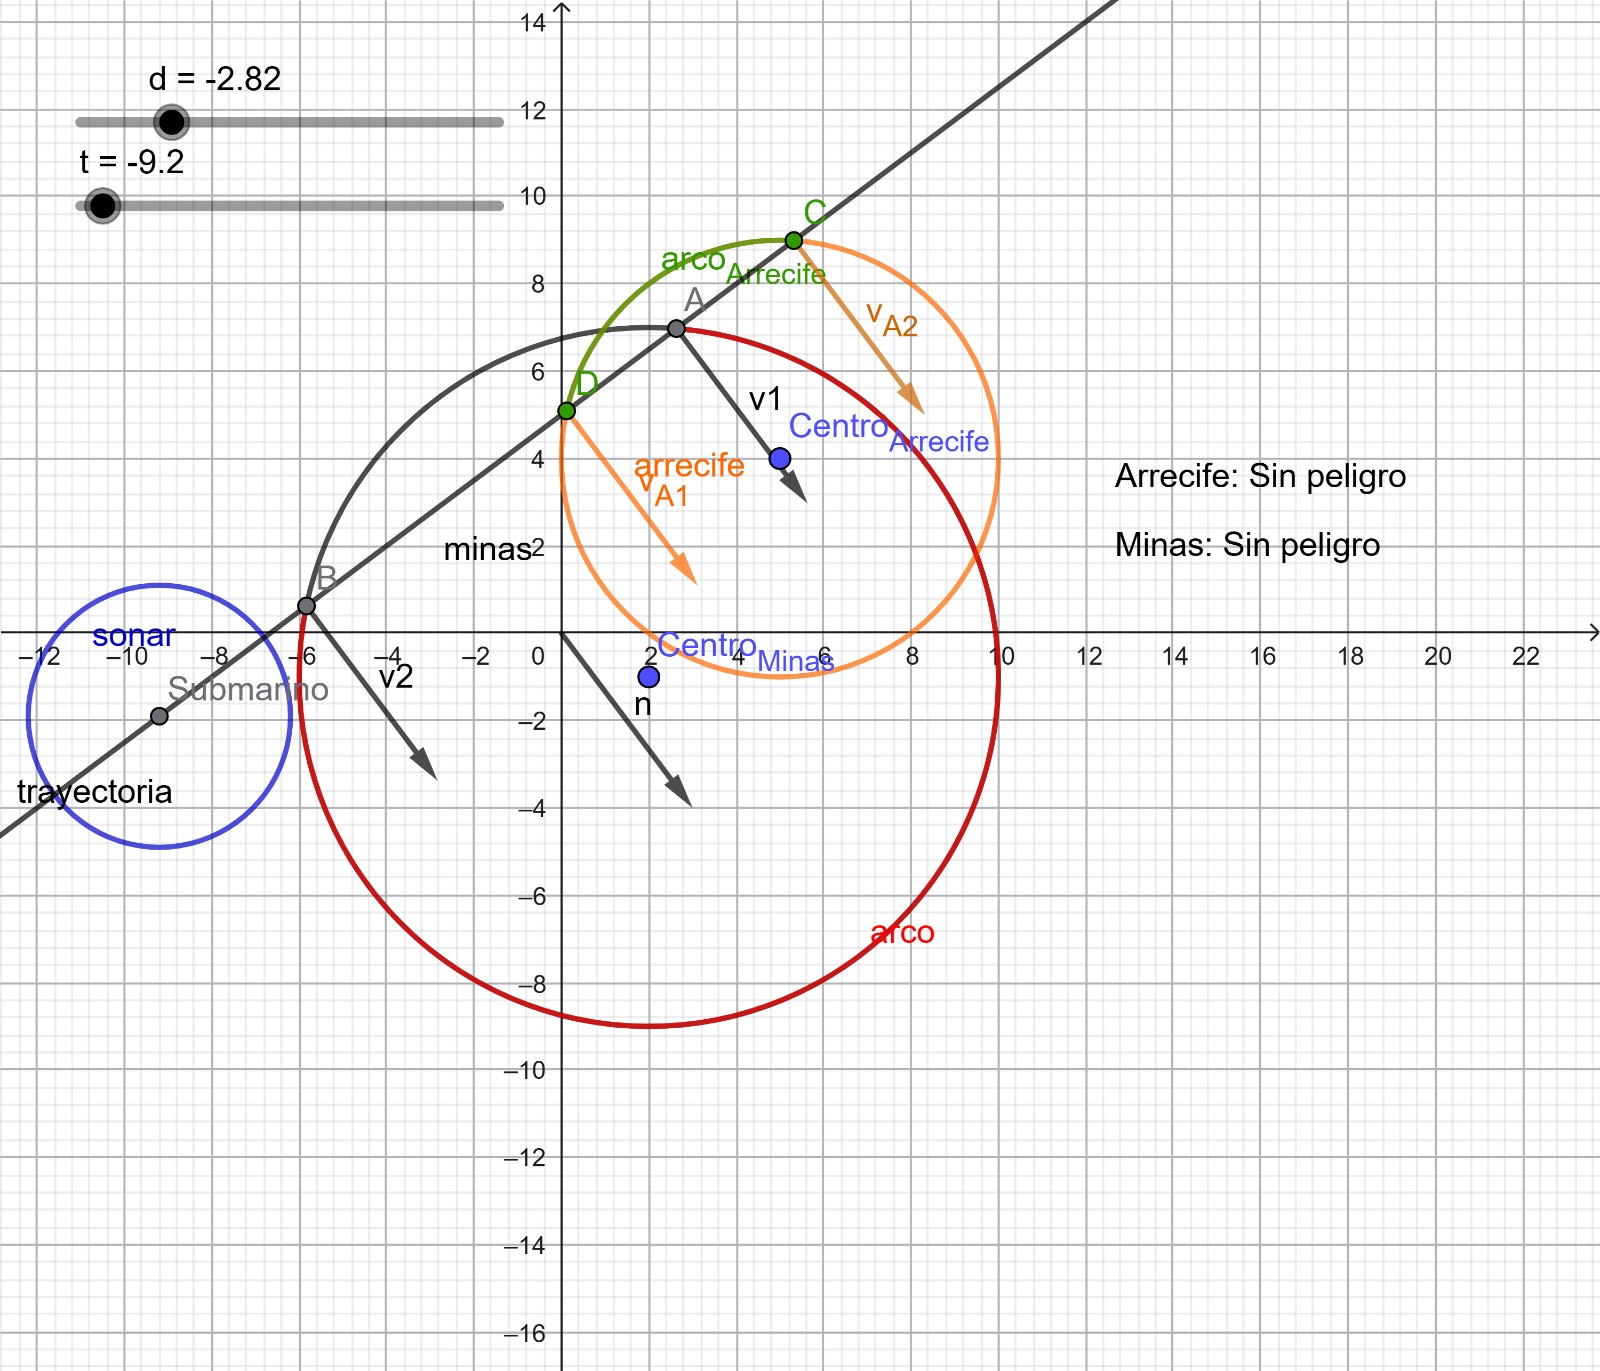
\includegraphics[height=6cm,keepaspectratio]{WhatsApp Image 2026-06-02 at 7.59.51 AM.jpeg}
    \vspace{0.1cm}
    
    \textit{\small Plano de Navegación en GeoGebra}
  \end{center}
\end{frame}

% --- DIAPOSITIVA 10: CONDICIÓN ANALÍTICA DE TANGENCIA ---
\begin{frame}{Problema I: Umbral de Tangencia y Seguridad}
  \begin{block}{Condición Analítica de Tangencia}
    Para que la trayectoria lineal del submarino $\ell$ sea exactamente tangente a la circunferencia del campo de minas centrado en $M(2, -1)$, el radio de exclusión $R$ debe igualar la distancia perpendicular mínima calculada en la Parte A:
    \[R_{\text{tangente}} = d_1 = 6\text{~km}\]
  \end{block}
  \vspace{0.4cm}
  \centering
  \small \textcolor{USSBlue}{\textbf{Definición Geométrica:} En este estado límite, el sistema de ecuaciones cuadrático-lineal tiene solución única, y la recta roza a la circunferencia en un único punto de coordenadas $(2, 7)$.}
\end{frame}

% --- DIAPOSITIVA 11: INTERPRETACIÓN DE SEGURIDAD NAVAL ---
\begin{frame}{Problema I: Interpretación de Seguridad Naval}
  \textbf{Análisis de Riesgo en el Contexto Táctico:}
  \vspace{0.3cm}
  \begin{itemize}
    \item \textbf{Alerta Mínima ($R = 6\text{~km}$):} 
      El submarino rozaría el límite del campo de minas en un único punto coordenado de contacto. Esto representa un margen de maniobra nulo ante derivas o corrientes marinas.
    \vspace{0.2cm}
    \item \textbf{Umbral Táctico de Navegación:}
      \begin{itemize}
        \item \textbf{Zona Segura ($R < 6\text{~km}$):} La trayectoria es \textbf{exterior} $\implies$ Tránsito 100\% libre de amenazas.
        \item \textbf{Zona de Incursión ($R > 6\text{~km}$):} La trayectoria es \textbf{secante} (como en el caso real $R = 8\text{~km}$) $\implies$ Penetración física en el campo minado.
      \end{itemize}
  \end{itemize}
\end{frame}

% --- NUEVA DIAPOSITIVA: TABLA DE RESULTADOS CONSOLIDADOS ---
\begin{frame}{Problema I: Resultados Consolidados de Telemetría}
  \centering
  \small
  \begin{tabular}{|l|c|c|}
    \hline
    \textbf{Parámetro Táctico} & \textbf{Modelo / Definición} & \textbf{Valor Calculado} \\
    \hline
    Trayectoria del submarino $\ell$ & Ecuación general de la recta & $3x - 4y + 20 = 0$ \\
    Centro del campo de minas & Coordenadas fijas $M(x_0, y_0)$ & $M(2, -1)$ \\
    Radio de exclusión de minas $R$ & Umbral de peligro físico & $8\text{~km}$ \\
    Distancia perpendicular $d_1$ & $d(M, \ell) = \frac{|3x_0 - 4y_0 + 20|}{5}$ & $\mathbf{6.0\text{~km}}$ \\
    Posición relativa (minas) & Criterio métrico: $d_1 < R$ & \textbf{Secante} (Incursión) \\
    \hline
    Centro del arrecife de coral & Coordenadas fijas $A(x_0, y_0)$ & $A(5, 4)$ \\
    Radio del arrecife $R_A$ & Umbral de peligro físico & $5\text{~km}$ \\
    Distancia perpendicular $d_2$ & $d(A, \ell) = \frac{|3x_0 - 4y_0 + 20|}{5}$ & $\mathbf{3.8\text{~km}}$ \\
    Posición relativa (arrecife) & Criterio métrico: $d_2 < R_A$ & \textbf{Secante} (Colisión) \\
    \hline
    Cuerda de peligro (minas) $L_1$ & $2\sqrt{R^2 - d_1^2}$ & $\mathbf{10.58\text{~km}}$ \\
    Cuerda de peligro (arrecife) $L_2$ & $2\sqrt{R_A^2 - d_2^2}$ & $\mathbf{6.50\text{~km}}$ \\
    Radio de tangencia límite & $R_{\text{tangente}} = d_1$ & $\mathbf{6.0\text{~km}}$ \\
    \hline
  \end{tabular}
\end{frame}


% 9. PROBLEMA I: CAPACIDAD Y COBERTURA DEL SONAR
\begin{frame}{Problema I: Capacidad y Cobertura del Sonar}
  El sonar del submarino tiene un alcance de telemetría acústica $R_s = 3\text{~km}$, formando una circunferencia móvil en torno a la posición instantánea del submarino $S$.
  \vspace{0.3cm}
  \begin{itemize}
    \item \textbf{Condición geométrica de contacto con el arrecife ($R_A = 5\text{~km}$):}
      \[d(S, A) \le R_s + R_A = 3 + 5 = 8\text{~km}\]
    \vspace{0.15cm}
    \item \textbf{Validación de Detección:}
      Como la distancia de máxima aproximación es $d_2 = 3.8\text{~km}$, y se cumple con holgura que:
      \[3.8\text{~km} \le 8\text{~km}\]
      \textbf{El sonar sí detectará el arrecife con total certeza}.
  \end{itemize}
\end{frame}

% 10. PROBLEMA I: INTERVALO Y PUNTOS DE ALERTA
\begin{frame}{Problema I: Intervalo y Puntos de Alerta del Sonar}
  \textbf{Cálculo del Tramo Total con Señal Activa ($L_{\text{det}}$):}
  \[L_{\text{det}} = 2\sqrt{(R_s + R_A)^2 - d_2^2} = 2\sqrt{8^2 - 3.8^2} \approx 14.08\text{~km}\]
  \vspace{0.2cm}
  \textbf{Coordenadas de Contacto Acústico en el Plano (Valores Exactos):}
  \[S_{1,2} \left( \frac{68 \pm 4\sqrt{1239}}{25}, \frac{176 \pm 3\sqrt{1239}}{25} \right)\]
  \vspace{0.15cm}
  \begin{itemize}
    \item \textbf{Punto de Inicio de Alerta ($S_1$):} $(-2.91, 2.82)$
    \item \textbf{Punto de Pérdida de Señal ($S_2$):} $(8.35, 11.26)$
  \end{itemize}
  \vspace{0.1cm}
  {\centering \scriptsize \textit{Esto proporciona $14.08\text{~km}$ continuos de telemetría de advertencia electrónica para maniobras evasivas.} \par}
\end{frame}

% 11. PROBLEMA I: SIMULACIÓN INTERACTIVA EN GEOGEBRA
\begin{frame}{Problema I: Simulación e Interactividad en GeoGebra}
  Para la validación de la navegación y las posiciones relativas, se implementó un modelo dinámico interactivo en GeoGebra:
  \vspace{0.3cm}
  \begin{itemize}
    \item \textbf{Enlace de Acceso:} \url{https://www.geogebra.org/classic/jasfmgg3}
    \vspace{0.2cm}
    \item \textbf{Control de Parámetros:} El modelo dispone de un deslizador $d_0$ que controla la ordenada al origen del trayecto lineal $y = 0.75x + d_0$.
    \vspace{0.2cm}
    \item \textbf{Interactividad Dinámica:} Al mover el deslizador, se simula en tiempo real la aproximación del submarino y se recalculan las posiciones relativas.
  \end{itemize}
\end{frame}

% --- NUEVA DIAPOSITIVA: ESCENARIOS DE ALERTA ---
\begin{frame}{Problema I: Escenarios de Alerta del Simulador}
  \centering
  \textbf{Apoyo Visual de Alerta en Tiempo Real en GeoGebra}
  \vspace{0.4cm}
  
  \begin{center}
  \begin{columns}[c]
    \begin{column}{0.60\textwidth}
      \centering
      \small
      \begin{tabular}{|l|c|l|}
        \hline
        \textbf{Escenario} & \textbf{Condición} & \textbf{Alerta en GeoGebra} \\
        \hline
        Secante & $d_0 < 7.5$ & Cuerda de peligro activa \\
        Tangente & $d_0 = 7.5$ & Contacto en un único punto \\
        Exterior & $d_0 > 7.5$ & Sin contacto (ruta segura) \\
        \hline
      \end{tabular}
    \end{column}
    \begin{column}{0.36\textwidth}
      \raggedright
      \scriptsize
    \end{column}
  \end{columns}
  \end{center}
\end{frame}

% 6. PROBLEMA I: PLANO DE NAVEGACIÓN (SOPORTE VISUAL)
\begin{frame}{Problema I: Plano de Navegación}
  \begin{center}
    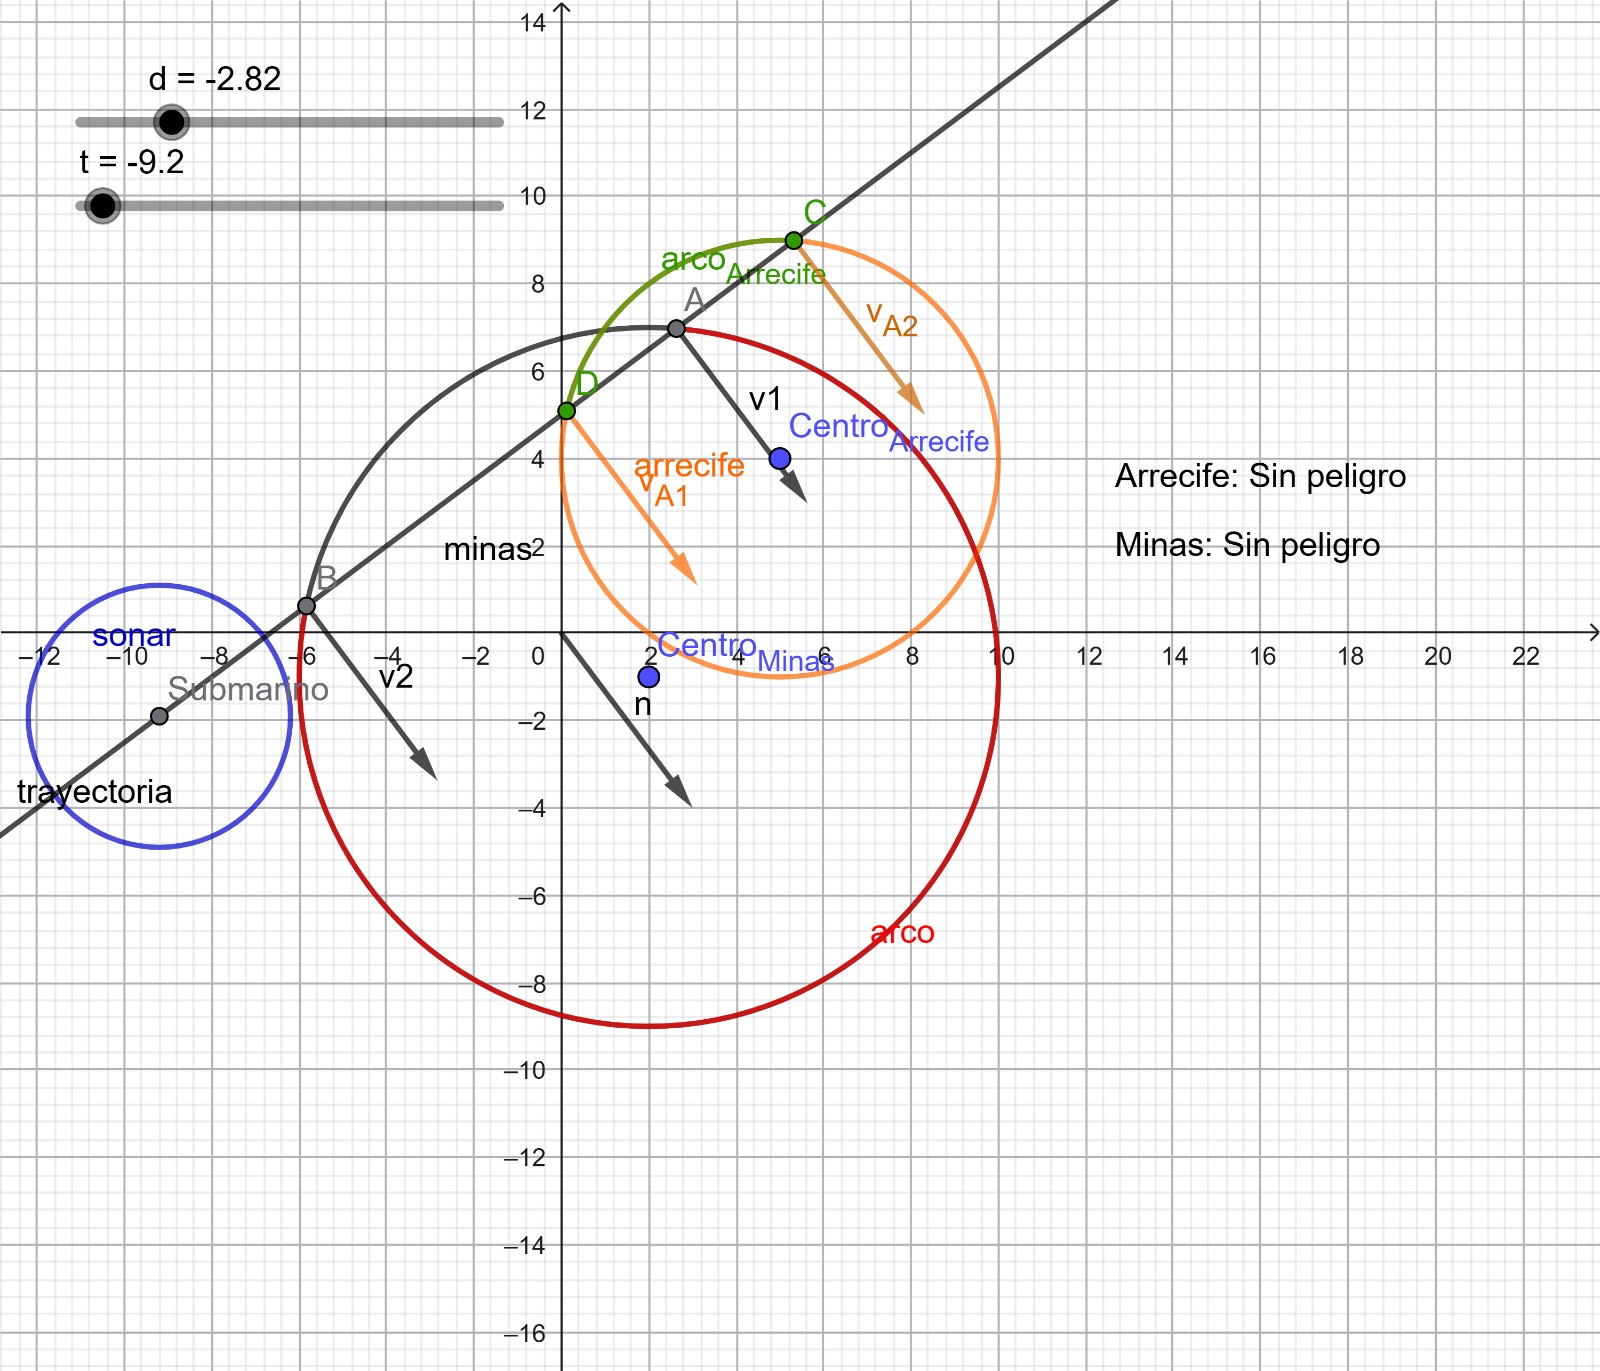
\includegraphics[height=6cm,keepaspectratio]{WhatsApp Image 2026-06-02 at 7.59.51 AM.jpeg}
    \vspace{0.1cm}
    
    \textit{\small Plano de Navegación en GeoGebra}
  \end{center}
\end{frame}


% 12. PROBLEMA I: ESCENARIOS DE VERIFICACIÓN EN GEOGEBRA
\begin{frame}{Problema I: Escenarios de Verificación en GeoGebra}
  \begin{columns}[T]
    \begin{column}{0.48\textwidth}
      \begin{center}
        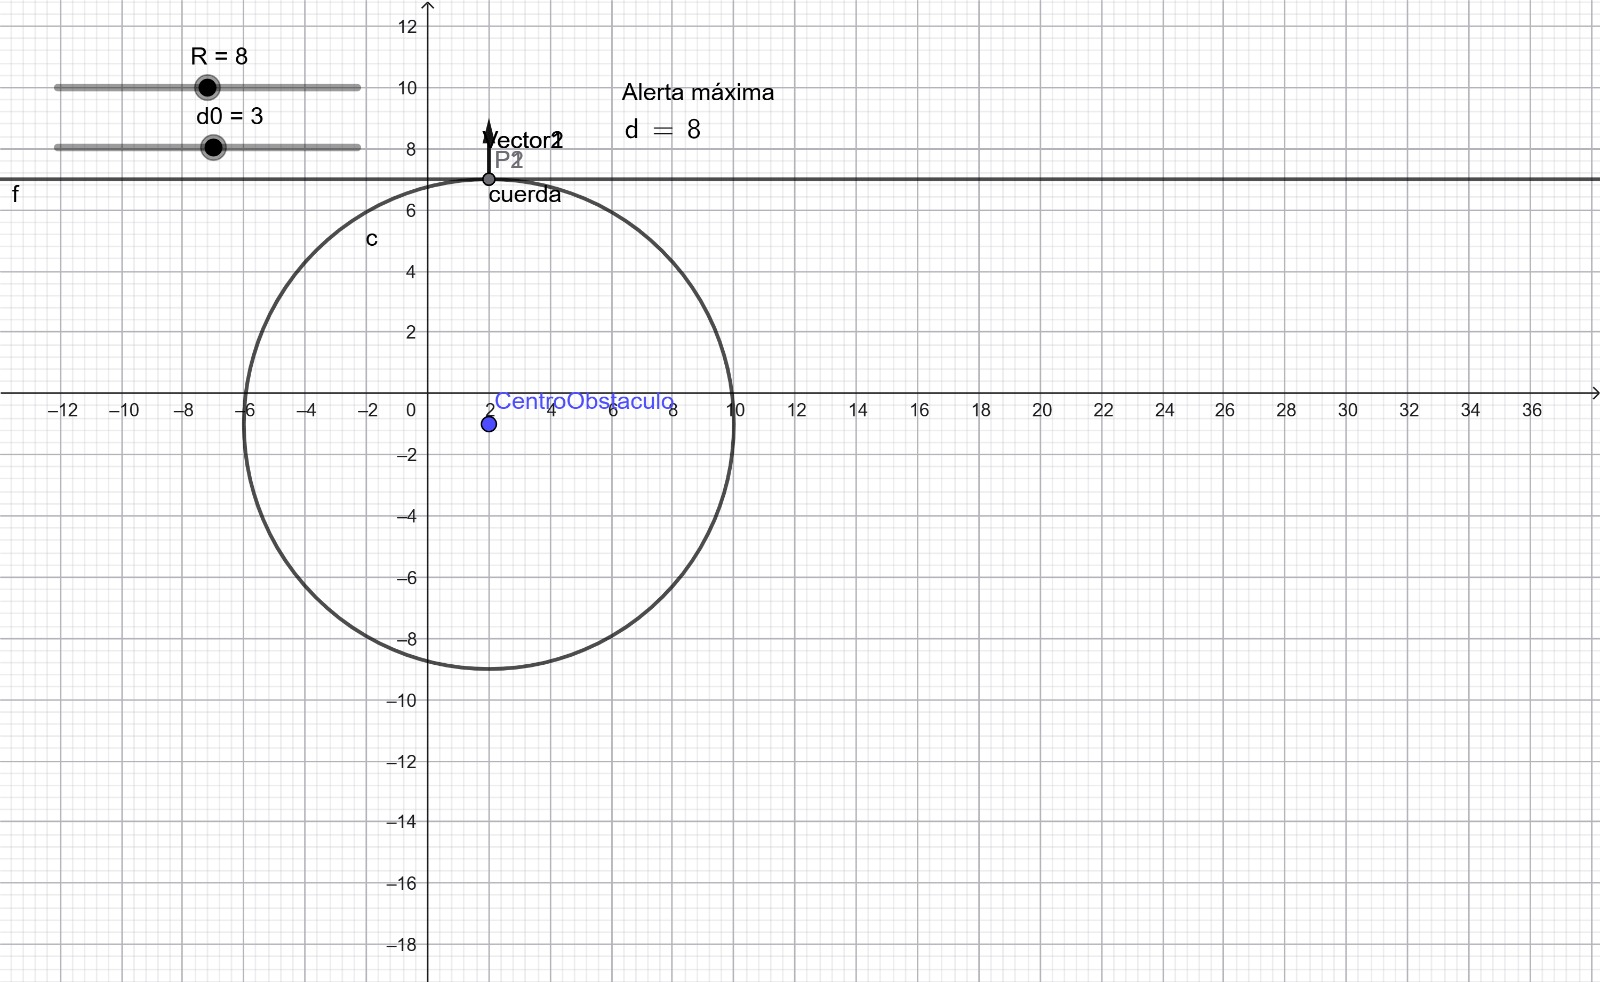
\includegraphics[width=0.98\textwidth]{WhatsApp Image 2026-06-02 at 7.52.09 AM.jpeg}
        \vspace{0.1cm}
        
        \scriptsize \textbf{Alerta Máxima ($d_0 < 7.5$):} El submarino cruza de forma secante ambos obstáculos. Cuerda de peligro roja activa.
      \end{center}
    \end{column}
    \begin{column}{0.48\textwidth}
      \begin{center}
        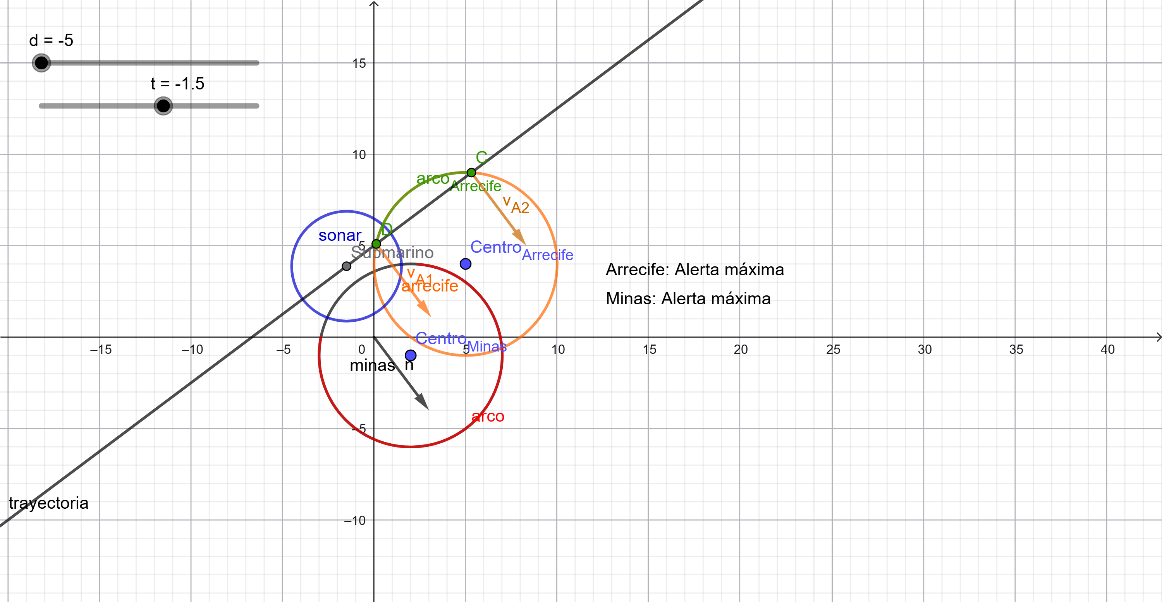
\includegraphics[width=0.98\textwidth]{image9.png}
        \vspace{0.1cm}
        
        \scriptsize \textbf{Ruta segura ($R = 5\text{~km}$):} Como $d_1 = 6\text{~km} > R_{\text{nuevo}} = 5\text{~km}$, la trayectoria pasa a ser \textbf{exterior}. La cuerda de peligro roja desaparece en GeoGebra, garantizando un tránsito seguro.
      \end{center}
    \end{column}
  \end{columns}
\end{frame}

% --- DIAPOSITIVA: PARTE D - REFLEXIÓN DE RUTA SEGURA ---
\begin{frame}{Problema I: Criterios Geométricos de Seguridad Naval}
  \begin{block}{Planificación de Rutas Submarinas Seguras}
    Para la seguridad naval en la planificación de rutas tácticas, los ingenieros deben evitar trayectorias \textbf{secantes} (peligro inminente de minas o encallamiento) y \textbf{tangentes} (margen de maniobra nulo).
  \end{block}
  \vspace{0.3cm}
  \textbf{Condición Matemática de Ruta Segura:}
  Para garantizar un tránsito seguro y libre de amenazas, la distancia ortogonal mínima $d$ a cada centro de peligro $C_i$ debe superar estrictamente su correspondiente radio de exclusión $R_i$:
  \[d(C_i, \ell) > R_i \quad \forall i \quad \implies \text{Posición Relativa Exterior}\]
  \vspace{0.2cm}
  \centering
  \scriptsize
  \textit{Esto asegura que el submarino navegue en todo momento por la zona exterior, anulando la probabilidad de contacto físico.}
\end{frame}

% --- DIAPOSITIVA: PARTE D - APLICACIONES EN INGENIERÍA ---
\begin{frame}{Problema I: Aplicaciones Civiles e Industriales de la Tangencia}
  \textbf{Otras Aplicaciones Prácticas de Posición Relativa Recta-Circunferencia:}
  \vspace{0.3cm}
  \begin{itemize}
    \item \textbf{Ingeniería Civil y Trazados Viales (Caso Tangente):}
      En el diseño de empalmes entre tramos rectos de carreteras y curvas circulares. Es imperativo que la calzada sea estrictamente \textbf{tangente} al arco circular. Esto evita quiebres direccionales bruscos en el volante y mitiga la fuerza centrífuga, previniendo accidentes.
    \vspace{0.2cm}
    \item \textbf{Telecomunicaciones y Antenas (Caso Secante / Exterior):}
      El área de cobertura de una antena radial define una circunferencia de radio $R$. Si un usuario viaja en línea recta (trayectoria lineal), la duración de la señal activa (\textbf{cuerda secante} $L$) ocurre únicamente cuando su distancia mínima es $d < R$, permitiendo modelar ventanas de comunicación estables.
  \end{itemize}
\end{frame}

% 14. PROBLEMA III: CONTEXTO Y JUSTIFICACIÓN AEROESPACIAL
\begin{frame}{Problema III: Contexto y Justificación Aeroespacial}
  \textbf{Modelamiento de Órbitas Cruzadas y Ventanas de Vuelo:}
  \vspace{0.3cm}
  \begin{itemize}
    \item \textbf{El Escenario:} En ingeniería aeroespacial, la Tierra se sitúa en el origen $O(0,0)$ como el cuerpo gravitatorio principal.
    \item \textbf{El Satélite (Elipse):} Describe una trayectoria cerrada, estable y periódica alrededor de la Tierra, representando la órbita de telemetría meteorológica.
    \item \textbf{La Sonda (Hipérbola):} Es lanzada desde la Tierra con una velocidad superior a la de escape, lo que la sitúa en una trayectoria abierta de exploración interplanetaria.
    \item \textbf{El Riesgo:} Al cruzarse las órbitas, es crítico determinar analíticamente los puntos exactos de intersección espacial. Esto permite definir la \textbf{ventana de lanzamiento}, de modo que la sonda sea lanzada cuando el satélite se encuentra en la porción opuesta de su elipse, anulando el riesgo de colisión.
  \end{itemize}
\end{frame}

% --- NUEVA DIAPOSITIVA: PLANTEAMIENTO DE PREGUNTAS (PROBLEMA III) ---
\begin{frame}{Problema III: Objetivos y Desafíos del Modelamiento Orbital}
  Para modelar el sistema y planificar de forma segura la ventana de lanzamiento, el equipo de dinámica de vuelo se plantea tres interrogantes clave a resolver:
  \vspace{0.4cm}
  \begin{enumerate}
    \item \textbf{Desafío I: Caracterización Analítica de las Órbitas} \\
      ¿Cuáles son las ecuaciones ordinarias y generales de la órbita elíptica del satélite y la trayectoria hiperbólica de la sonda espacial, y cuáles son las coordenadas de sus focos y asíntotas bajo concurrencia focal recíproca?
    \vspace{0.2cm}
    \item \textbf{Desafío II: Determinación de Puntos de Interferencia Espacial} \\
      ¿Cuáles son las coordenadas cartesianas exactas de los puntos comunes de intersección entre la elipse y la hipérbola y qué interpretación física representan para la seguridad aeroespacial?
    \vspace{0.2cm}
    \item \textbf{Desafío III: Análisis Paramétrico y Simulación Dinámica} \\
      ¿Cómo se comportan las órbitas y las intersecciones al variar la excentricidad de la hipérbola y qué condiciones paramétricas garantizan la tangencia límite?
  \end{enumerate}
\end{frame}

% 15. PROBLEMA III: ELEMENTOS DE LA ÓRBITA ELÍPTICA
\begin{frame}{Problema III: Elementos de la Órbita Elíptica}
  El satélite meteorológico describe una órbita elíptica horizontal $\mathcal{E}$ de ecuación ordinaria:
  \[\mathcal{E} \colon \frac{x^2}{25} + \frac{y^2}{16} = 1\]
  \vspace{0.2cm}
  \begin{itemize}
    \item \textbf{Semiejes de la Elipse:}
      \[a_{\mathcal{E}} = 5\text{~u} \quad (50.000\text{~km}), \quad b_{\mathcal{E}} = 4\text{~u} \quad (40.000\text{~km})\]
    \item \textbf{Cálculo de la Distancia Focal de la Elipse ($c_{\mathcal{E}}$):}
      \[c_{\mathcal{E}} = \sqrt{a_{\mathcal{E}}^2 - b_{\mathcal{E}}^2} = \sqrt{25 - 16} = \sqrt{9} = 3\text{~u}\]
    \item \textbf{Coordenadas Coincidentes de los Focos ($\mathcal{E}$):}
      $F_1(-3, 0)$ y $F_2(3, 0)$
  \end{itemize}
\end{frame}

% 16. PROBLEMA III: ÓRBITA DE LA SONDA HIPERBÓLICA
\begin{frame}{Problema III: Órbita de la Sonda Hiperbólica}
  Por exigencias de la misión, se establece una \textbf{concurrencia focal recíproca} con $c_{\mathcal{H}} = 5$:
  \vspace{0.2cm}
  \begin{itemize}
    \item \textbf{Semieje real ($a_{\mathcal{H}}$):} Los vértices de la hipérbola coinciden con los focos de la elipse $\implies a_{\mathcal{H}} = c_{\mathcal{E}} = 3$.
    \item \textbf{Cálculo del semieje imaginario ($b_{\mathcal{H}}$):}
      \[b_{\mathcal{H}}^2 = c_{\mathcal{H}}^2 - a_{\mathcal{H}}^2 = 5^2 - 3^2 = 25 - 9 = 16 \implies b_{\mathcal{H}} = 4\]
    \item \textbf{Ecuación canónica resultante de la sonda ($\mathcal{H}$):}
      \[\mathcal{H} \colon \frac{x^2}{9} - \frac{y^2}{16} = 1\]
    \item \textbf{Asíntotas lineales de escape de la sonda:}
      \[y = \pm \frac{4}{3}x\]
  \end{itemize}
\end{frame}

% 17. PROBLEMA III: RESOLUCIÓN DEL SISTEMA CUADRÁTICO
\begin{frame}{Problema III: Intersección Analítica de Órbitas}
  Para hallar los puntos de cruce en el plano orbital, planteamos el sistema cuadrático de segundo grado:
  \begin{align*}
    16x^2 + 25y^2 &= 400 \quad (1) \\
    16x^2 - 9y^2 &= 144 \quad (2)
  \end{align*}
  \vspace{0.2cm}
  \textbf{Resolución por el método de reducción (restando la ecuación (2) a la (1)):}
  \[(16x^2 + 25y^2) - (16x^2 - 9y^2) = 400 - 144\]
  \[34y^2 = 256 \implies y^2 = \frac{128}{17} \approx 7.53\]
  \[y = \pm \sqrt{\frac{128}{17}} = \pm \frac{8\sqrt{34}}{17} \approx \pm 2.74\]
\end{frame}

% 18. PROBLEMA III: COORDENADAS DE INTERSECCIÓN
\begin{frame}{Problema III: Coordenadas de Colisión Orbital}
  \textbf{Sustituyendo $y^2 = \frac{128}{17}$ en la ecuación (2) para despejar la abscisa $x$:}
  \[16x^2 - 9\left(\frac{128}{17}\right) = 144 \implies 16x^2 = \frac{3600}{17} \implies x^2 = \frac{225}{17} \implies x = \pm \frac{15\sqrt{17}}{17}\]
  \vspace{0.25cm}
  \textbf{Cuatro Puntos de Intersección Analíticos Exactos:}
  \[I \left( \pm \frac{15\sqrt{17}}{17}, \pm \frac{8\sqrt{34}}{17} \right) \approx (\pm 3.64, \pm 2.74) \quad \text{(escala } 10.000\text{ km)}\]
  \vspace{0.2cm}
  {\centering \scriptsize \textit{Estas coordenadas de intersección simétrica definen las zonas de riesgo máximo de impacto orbital, fundamentales para calcular la ventana de lanzamiento de la sonda.} \par}
\end{frame}

% 19. PROBLEMA III: PLANO AEROESPACIAL (SOPORTE VISUAL)
\begin{frame}{Problema III: Plano del Sistema Aeroespacial}
  \begin{center}
    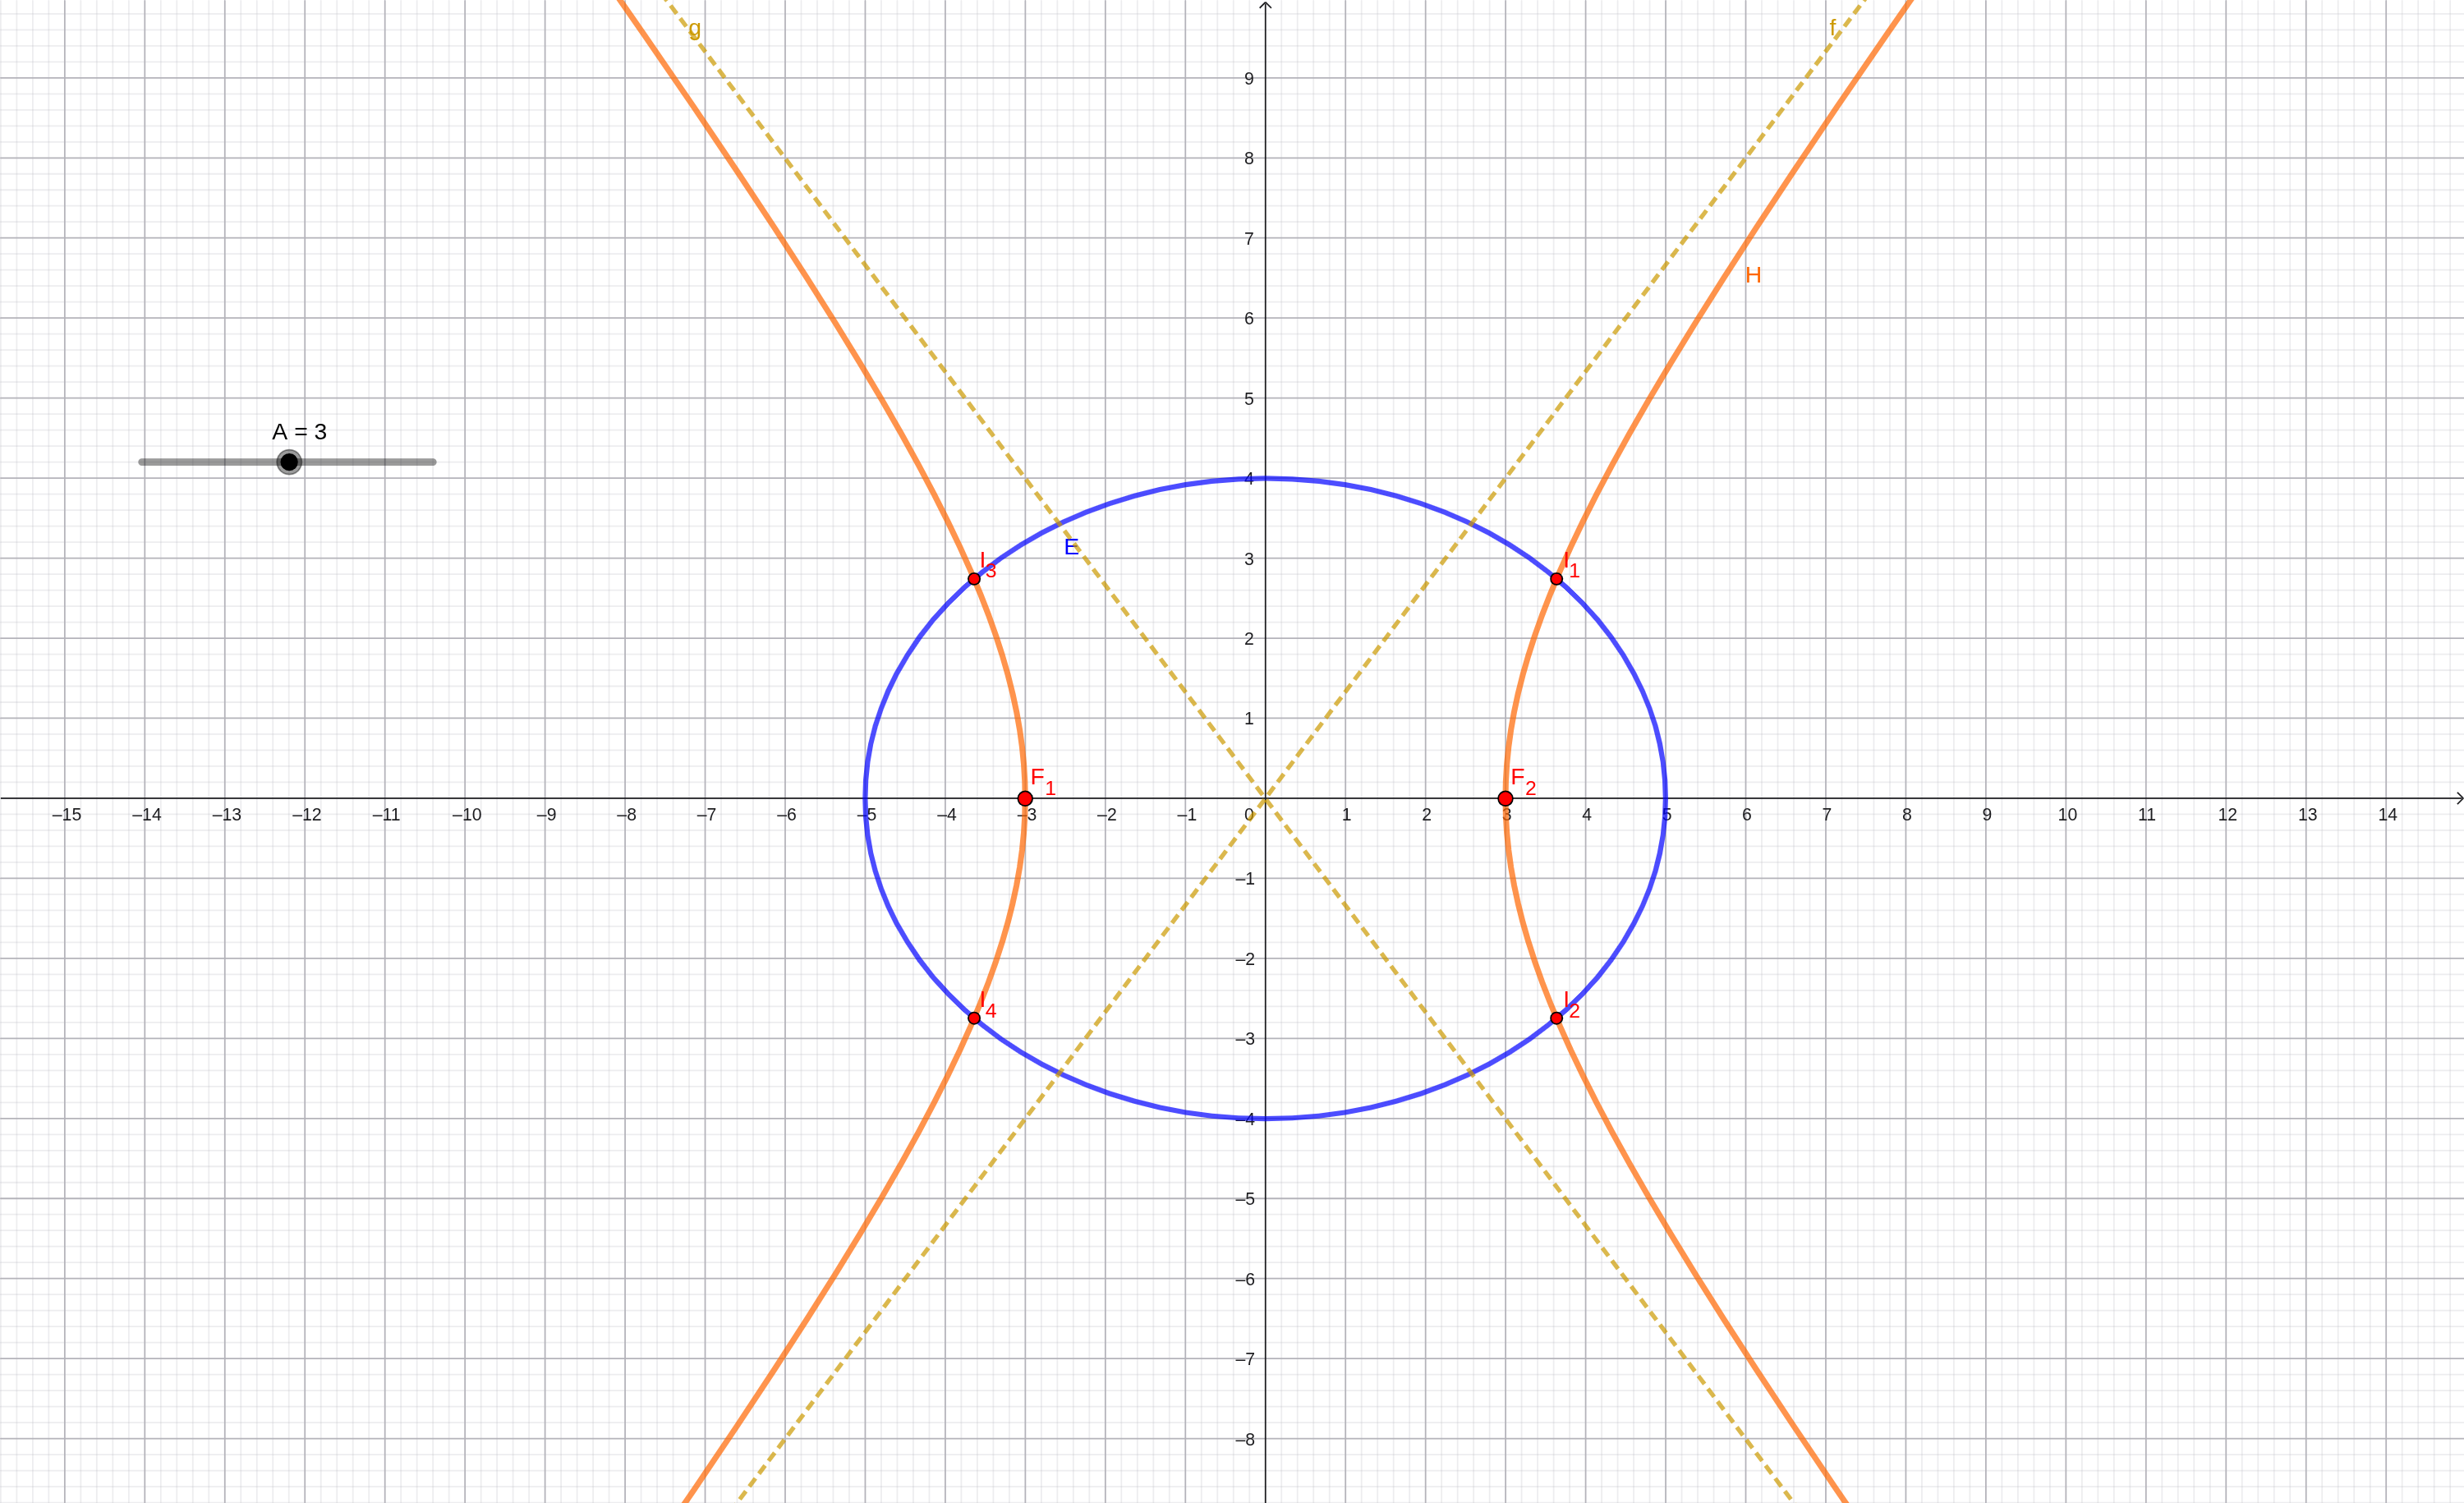
\includegraphics[height=6.2cm,keepaspectratio]{geogebra_problema3.png}
    \vspace{0.1cm}
    
    \textit{\small Plano Cartesiano Aeroespacial en GeoGebra: Intersección de la elipse orbital del satélite (azul), la trayectoria hiperbólica de escape (naranja), sus asíntotas y los 4 puntos de colisión simétricos.}
  \end{center}
\end{frame}

% 20. PROBLEMA III: EXCENTRICIDAD Y DINÁMICA ORBITAL
\begin{frame}{Problema III: Excentricidad y Dinámica Orbital}
  \centering
  \textbf{Excentricidad y Comportamiento Dinámico de las Órbitas:}
  \vspace{0.4cm}
  
  \begin{tabular}{|l|c|l|}
    \hline
    \textbf{Cónica} & \textbf{Excentricidad ($e$)} & \textbf{Comportamiento Dinámico} \\
    \hline
    Elipse $\mathcal{E}$ & $e_{\mathcal{E}} = \frac{c_{\mathcal{E}}}{a_{\mathcal{E}}} = \frac{3}{5} = 0.60$ & Trayectoria elíptica cerrada, estable y periódica \\
    \hline
    Hipérbola $\mathcal{H}$ & $e_{\mathcal{H}} = \frac{c_{\mathcal{H}}}{a_{\mathcal{H}}} = \frac{5}{3} \approx 1.67$ & Trayectoria hiperbólica abierta y escape veloz \\
    \hline
  \end{tabular}
  \vspace{0.4cm}
  \raggedright
  \small
  \begin{itemize}
    \item \textbf{Elipse ($e < 1$):} Modela el movimiento elíptico cerrado y periódico del satélite meteorológico terrestre.
    \item \textbf{Hipérbola ($e > 1$):} Representa la trayectoria de escape abierta y no periódica de la sonda hacia el espacio profundo.
  \end{itemize}
\end{frame}

% --- NUEVA DIAPOSITIVA: ANALISIS DE VARIACIÓN PARAMÉTRICA ---
\begin{frame}{Problema III: Análisis de Variación Paramétrica}
  \textbf{Efectos de la Velocidad de Escape ($c_{\mathcal{H}} = 5$ Constante):}
  \vspace{0.2cm}
  \begin{itemize}
    \item \textbf{Menor Velocidad (Menor Excentricidad $e_{\mathcal{H}} \to 1$):} \\
      El semieje real $a_{\mathcal{H}}$ aumenta y la hipérbola se ensancha horizontalmente. En el límite $a_{\mathcal{H}} \to 5$, las cuatro intersecciones convergen en dos puntos de tangencia horizontal: $T_{1,2}(\pm 5, 0)$.
    \vspace{0.2cm}
    \item \textbf{Mayor Velocidad (Mayor Excentricidad $e_{\mathcal{H}} \to \infty$):} \\
      El semieje real $a_{\mathcal{H}} \to 0$ y el semieje imaginario $b_{\mathcal{H}} \to 5$. Geométricamente, la hipérbola se \textbf{estrecha horizontalmente} ($2a_{\mathcal{H}} \to 0$) y se expande verticalmente, haciendo que las cuatro intersecciones converjan hacia los extremos de la elipse sobre el eje $y$: $I_v(0, \pm 4)$.
  \end{itemize}
\end{frame}

% 21. PROBLEMA III: SIMULADOR INTERACTIVO EN GEOGEBRA
\begin{frame}{Problema III: Simulador Orbital en GeoGebra}
  Para la validación de las órbitas y el cálculo de intersecciones dinámicas, se desarrolló un modelo dinámico interactivo en GeoGebra:
  \vspace{0.3cm}
  \begin{itemize}
    \item \textbf{Enlace de Acceso:} \url{https://www.geogebra.org/classic/dmqg3c7k}
    \item \textbf{Control de Parámetros:} El modelo dispone de un deslizador $a_{\mathcal{H}}$ que permite variar en tiempo real el semieje real de la trayectoria hiperbólica en el rango $[1.00, 4.95]$.
    \item \textbf{Física de Escape:} Al mover el deslizador, se visualiza la variación de la excentricidad orbital y el desplazamiento instantáneo de los 4 puntos de colisión sobre la elipse.
  \end{itemize}
\end{frame}

% 23. CONCLUSIÓN GENERAL
\begin{frame}{Conclusión General}
  \begin{itemize}
    \item \textbf{Trascendencia del Rigor Analítico:} Las cónicas modelan de forma matemática fenómenos físicos reales donde la precisión métrica dota de viabilidad y seguridad a las operaciones complejas.
    \item \textbf{Táctica y Telemetría Naval:} La posición relativa recta-circunferencia y el estudio de las cuerdas de peligro evitan catástrofes en la planificación del tránsito de naves submarinas.
    \item \textbf{Dinámica y Balística Celeste:} Las cónicas recíprocas concurrentes permiten predecir zonas de impacto y coordinar ventanas seguras de lanzamiento interplanetario.
    \item \textbf{Soporte Tecnológico:} Herramientas como GeoGebra resultan fundamentales en ingeniería civil y aeroespacial para simular, verificar y validar modelos con bases analíticas sólidas.
  \end{itemize}
\end{frame}

% --- NUEVA DIAPOSITIVA: REFERENCIAS BIBLIOGRÁFICAS ---
\begin{frame}{Referencias Bibliográficas}
  \scriptsize
  \begin{thebibliography}{9}
    \bibitem{larson}
    Larson, R. (2018). \textit{Precálculo} (10.ª ed.). Cengage Learning.
    
    \bibitem{stewart}
    Stewart, J., Redlin, L., y Watson, S. (2016). \textit{Precálculo: Matemáticas para el cálculo} (7.ª ed.). Cengage Learning.
    
    \bibitem{curtis}
    Curtis, H. D. (2020). \textit{Orbital mechanics for engineering students} (4.ª ed.). Butterworth-Heinemann.
    
    \bibitem{geogebra}
    GeoGebra. (2026). \textit{GeoGebra Classic} (Versión 6.0) [Software de computación gráfica]. https://www.geogebra.org
  \end{thebibliography}
\end{frame}

% 24. AGRADECIMIENTOS
\begin{frame}
  \begin{center}
    
\includegraphics[width=3.8cm]{logo_uss.png}
    \vspace{0.5cm}
    
    \Large \color{USSBlue} \textbf{¡Muchas gracias por su atención!}
    \vspace{0.4cm}
    
    \small Introducción al Cálculo --- Facultad de Ingeniería \\ Universidad San Sebastián, 2026.
  \end{center}
\end{frame}

\end{document}
